%%%%%%%%%%%%%%%%%%%%%%%%%%%%%%%%%%%%%%%%%
% a0poster Portrait Poster
% LaTeX Template
% Version 1.0 (22/06/13)
%
% The a0poster class was created by:
% Gerlinde Kettl and Matthias Weiser (tex@kettl.de)
% 
% This template has been downloaded from:
% http://www.LaTeXTemplates.com
%
% License:
% CC BY-NC-SA 3.0 (http://creativecommons.org/licenses/by-nc-sa/3.0/)
%
%%%%%%%%%%%%%%%%%%%%%%%%%%%%%%%%%%%%%%%%%

%----------------------------------------------------------------------------------------
%	PACKAGES AND OTHER DOCUMENT CONFIGURATIONS
%----------------------------------------------------------------------------------------

\documentclass[a0,portrait]{a0poster}

\usepackage{multicol} % This is so we can have multiple columns of text side-by-side
\columnsep=100pt % This is the amount of white space between the columns in the poster
\columnseprule=5pt % This is the thickness of the black line between the columns in the poster

\usepackage[svgnames]{xcolor} % Specify colors by their 'svgnames', for a full list of all colors available see here: http://www.latextemplates.com/svgnames-colors

\usepackage{times} % Use the times font
%\usepackage{palatino} % Uncomment to use the Palatino font

\usepackage{graphicx} % Required for including images
\graphicspath{{figures/}} % Location of the graphics files
\usepackage{booktabs} % Top and bottom rules for table
\usepackage[font=small,labelfont=bf]{caption} % Required for specifying captions to tables and figures
\usepackage{amsfonts, amsmath, amsthm, amssymb} % For math fonts, symbols and environments
\usepackage{wrapfig} % Allows wrapping text around tables and figures

\begin{document}

%----------------------------------------------------------------------------------------
%	POSTER HEADER 
%----------------------------------------------------------------------------------------

% The header is divided into two boxes:
% The first is 75% wide and houses the title, subtitle, names, university/organization and contact information
% The second is 25% wide and houses a logo for your university/organization or a photo of you
% The widths of these boxes can be easily edited to accommodate your content as you see fit

\begin{minipage}[b]{0.8\linewidth}
\color{NavyBlue} \VeryHuge{\textbf{Digitalne urbane mreže i društveni mediji}} 
\color{Black}\\ % Title

\huge \textbf{Tamara Jevtimijević, 261/2017}\\[0.5cm] % Author(s)
\huge Računarstvo i društvo, Matematički fakultet u Beogradu\\[0.4cm] % University/organization
\Large \textit{Email: mi17261@alas.matf.bg.ac.rs}\\
\end{minipage}
%
\begin{minipage}[b]{0.2\linewidth}
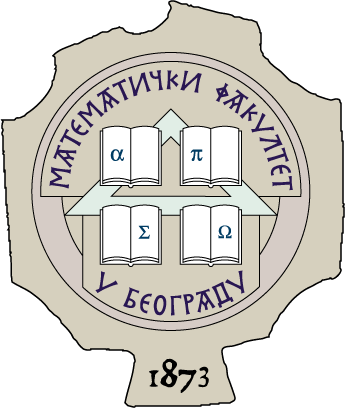
\includegraphics[width=12cm]{logo.png}\\
\end{minipage}

\vspace{3cm} % A bit of extra whitespace between the header and poster content

%----------------------------------------------------------------------------------------

\begin{multicols}{2} % This is how many columns your poster will be broken into, a portrait poster is generally split into 2 columns

%----------------------------------------------------------------------------------------
%	ABSTRACT
%----------------------------------------------------------------------------------------

\color{Black} % Navy color for the abstract


%----------------------------------------------------------------------------------------
%	INTRODUCTION
%----------------------------------------------------------------------------------------

\color{Black} % SaddleBrown color for the introduction

\section*{\Huge{Uvod}}

\Large{
Krajem dvadesetog i početkom dvadeset prvog veka informaciono-komunikacione korporacije su doživele najveću ekspanziju. Danas ih ima sve više i sve su više uticajne. Tehnologija je uznapredovala velikom brzinom i svoje grane je pustila svuda. Danas gde god da se okrenemo digitalizacija je oko nas. 
}

%----------------------------------------------------------------------------------------
%	OBJECTIVES
%----------------------------------------------------------------------------------------

\color{teal} % DarkSlateGray color for the rest of the content

\section*{\huge{\textit{Teme:}}}

\begin{enumerate}
\item \textit{Statistike napredovanja pametnih gradova kroz monopol.}
\item \textit{Rešavanje problema stranih start-apova.}
\item \textit{Digitalna urbana infrastruktura.}
\item \textit{Uspon informaciono - komunikacionih tehnologija.}
\item \textit{Monopol IKT-a.}
\item \textit{Društvene mreže i grad.}
\item \textit{Urbano brendiranje i društvene mreže.}
\end{enumerate}

%----------------------------------------------------------------------------------------
%	MATERIALS AND METHODS
%----------------------------------------------------------------------------------------

\color{black}

\section*{\Huge{Društvene mreže i grad}}

\Large{
Uspon društvenih mreža kao što su Facebook, Twitter, WeChat, Tumblr, Instagram, Google+, YouTube, Linkedin, TikTok, Snapchat i WhatsApp promenio je način na koji ljudi širom sveta komuniciraju i žive. Čini se da ljudi više vole i primenjuju digitalne interakcije u odnosu na fizičke interakcije. 
Procenjuje se da preko 3,2 milijarde ljudi širom sveta koristite društvene mreže na ovaj ili onaj način, a ovi trendovi su zaslužni za širok prodor pametnih uređaja kao što su mobilni telefoni i tableti.
}

\begin{center}\vspace{2cm}
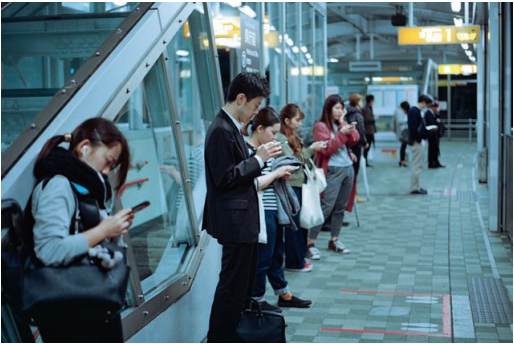
\includegraphics[width=35cm,height=25cm]{mreze.png}
\end{center}\vspace{12cm}

\section*{\Huge{Urbano brendiranje i društvene mreže}}

\Large{
Pojava digitalnih rešenja, koja se fokusiraju na gradove i urbana područja je imala brojne pozitivne strane, kao što je mogućnost brendiranja grada. Digitalni brend je dao gradovima priliku da digitalne tehnologije iskoriste na ekonomskoj granici. Nakon pojave društvenih mreža, turistički brendovi su prihvaćeni u različitim gradovima. Brendiranje je strategija koja je nevino usvojena, da bi se oni, koji žive u nekom gradu i u njemu rade, ali i oni koji su ga samo posetili osetili njegovim delom.
}

\begin{center}\vspace{1cm}
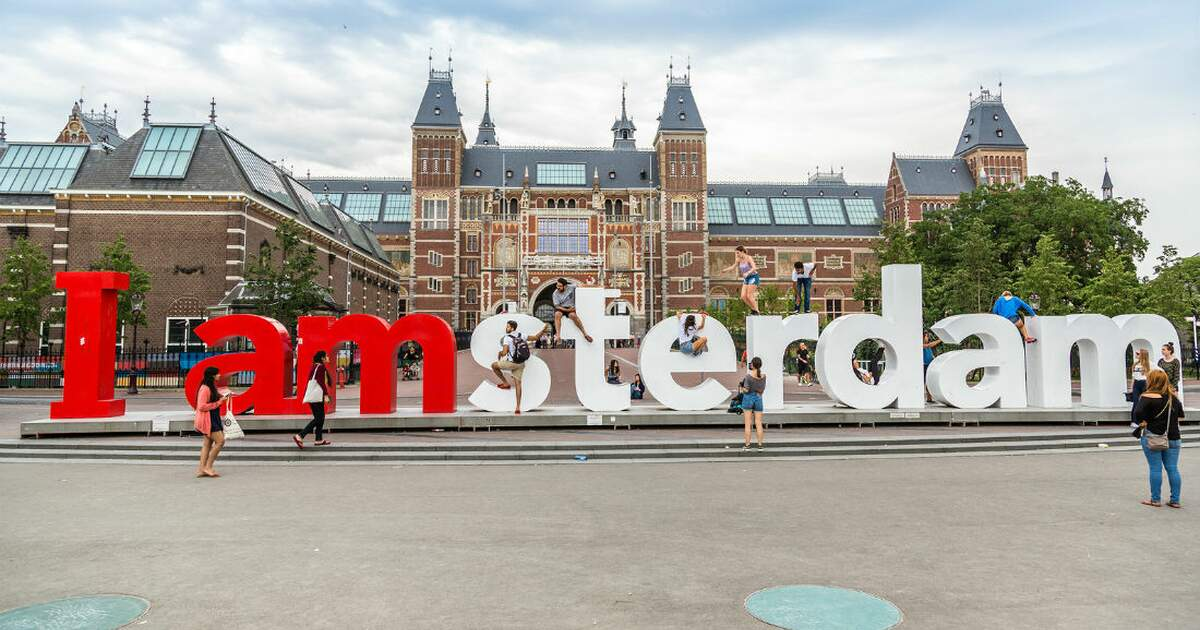
\includegraphics[width=30cm,height=20cm]{rijksmuseum-amsterdam-museum-iamsterdam.jpg}
\end{center}\vspace{1cm}

\begin{center}\vspace{1cm}

\includegraphics[width=30cm,height=25cm]{Quinonez_Julian_Istanbul_Logo.png}
\end{center}\vspace{1cm}

%----------------------------------------------------------------------------------------
%	CONCLUSIONS
%----------------------------------------------------------------------------------------

\color{SaddleBrown} % SaddleBrown color for the conclusions to make them stand out

\color{teal}

\section*{\huge{Zaključak}}

\Large{
Možemo primetiti sve veću ulogu digitalnih medija u
oblikovanju gradske privrede i političke sfere. Uloga društvenih medija, odnosno mreža u gradovima, posebno u javnim prostorima, postaje sve više naglašena. Vidi se da političari sve više koriste društvene platforme, kako bi stekli političku kilometražu i ekonomsku otpornost, kroz povećanje aktivnosti u vezi sa turizmom korišćenjem novih tehnika brendiranja i marketinga.
}

\end{multicols}
\end{document}